\capitulo{3}{Conceptos teóricos}

En esta sección vamos a explicar los algoritmos utilizados en el desarrollo del proyecto. Primero veremos los algoritmos relativos a la planificación de la ruta, y a continuación aquellos relativos al seguimiento de la misma de una forma autónoma por parte del vehículo.

\section{Algoritmo \Astar}

\Astar es un algoritmo de búsqueda informada del tipo primero el mejor, que usa una función de evaluación para elegir hacia que nodo expandirse desde un nodo inicial hacia un nodo final.

Para representar el espacio de búsqueda del algoritmo, se usa una cuadrícula, es por lo tanto un algoritmo que opera en un espacio de estados discreto. Cada nodo de la cuadrícula puede representar un espacio donde es posible desplazarse o un obstáculo que es inalcanzable.

La función F() de evaluación calcula el coste de cada nodo, con lo que se eligen los nodos con menor coste para llegar al destino a través del camino óptimo. Esta función está a su vez formada por dos funciones: una función G() que calcula el coste del camino seguido desde el nodo inicial a ese nodo concreto, y una función H() o función heurística que hace una estimación del coste del camino desde ese nodo al nodo final o meta.

El algoritmo comienza desde el nodo inicial explorando los nodos adyacentes o sucesores. Un nodo ya explorado, es decir del que ya se ha buscado sus sucesores, se manda a la lista de nodos cerrados. Con los sucesores se forma una lista de nodos abiertos o por explorar, de la cual se elige el de menor coste para ser el siguiente en ser explorado, hasta que se alcance el nodo meta o no queden más nodos por ser explorados (si no quedasen más nodos significaría que no hay un camino entre el nodo inicial y la meta). Si al explorar un nodo esta ya se encontraba en alguna de las listas de nodos abiertos o cerrados, se actualizarán los valores de los nodos al de menor coste encontrado.

\subsubsection{Heurística} \label{heuristicaaestrella}
El algoritmo \Astar es completo, lo que significa que encontrará un camino hasta la meta siempre que este exista. Además, para que sea admisible, que significa que siempre encontrará un camino óptimo, su función H() también debe ser admisible.

Una función H() es admisible siempre y cuando no sobrestime el coste del camino desde un nodo hasta la meta. Por ejemplo, se puede considerar que el camino desde un nodo hasta la meta será la línea recta.

La admisibilidad del \Astar trae consigo un gran coste computacional debido al gran número de nodos explorados. Para mejorar la eficiencia podemos dar pesos a las funciones G() y H(), de tal forma que si damos más valor a G() la búsqueda se expandirá en anchura buscando el camino, mientras que si damos más valor a H() se expandirá más rápido acercándose a la meta.

Para el \Astar y algunas de sus variantes, el Theta* \ref{referenciaTheta} y el \Astar con vértices \ref{avertices}, hemos usado la distancia euclídea, tanto para la función G(), como para la función H(). La función G() es la distancia recorrida desde el inicio hasta ese punto, y la función H() es la distancia en línea recta desde donde nos encontremos a la meta.

\subsection{Pseudocódigo \Astar}
\scalebox{1.0}{
\begin{algorithm}[H]
 abiertos = cerrados = $\O$\;
 actual = inicio\;
 abiertos.añadir(actual, actual.coste)\;

 \While{abiertos no esté vacío}{
  actual = abiertos.primerElemento()\;
  cerrados.añadir (actual)\;
  
  \eIf{actual es la meta}{
    \nl\KwRet{Camino encontrado}
  }{
    sucesores = obtenerSucesores(actual)\;
    
    \ForAll{los sucesores de actual} {
        \If {sucesor está en abiertos}{
            \If {coste en abiertos es mayor que el del sucesor}{
				abiertos.actualizar (actual, actual.coste)\;	
            }		
        }
        
        \If {sucesor está en cerrados}{
            \If {coste en cerrados es mayor que el del sucesor}{
				cerrados.borrar (actual)\;	
				abiertos.añadir (actual)\;
            }
        }
        
        \If {sucesor no está ni en abiertos ni en cerrado}{
		        abiertos.añadir (actual)\;
        }
    } 
  }
 }
 \nl\KwRet{Error: Camino no encontrado}
 \caption{Pseudocódigo del \Astar}
\end{algorithm}
}

\section{\textit{Path Smoothing} o Suavizado}

Un problema del \Astar tradicional es que las rutas que encuentra, aunque sean las más cortas, no tienen una apariencia realista. Esto es debido a que el \Astar discretiza el espacio de búsqueda para poder buscar la ruta. Dependiendo de la representación que elijamos, se acercará más a o menos a la realidad, pero en cualquier caso se producirá una diferencia que suele estar alejada de la representación ideal de esa misma ruta.

Por ejemplo, en el caso de una búsqueda en una cuadrícula, si seguimos el camino a través de cada casilla, cuando el camino siga una ruta en diagonal, el \Astar seguirá un camino en zigzag. Aunque este camino es perfectamente válido, en la realidad no se sigue un camino en zigzag si no que se sigue la línea recta que representa. En el caso de las curvas el problema es parecido. El camino encontrado estará formado por segmentos rectos en vez de seguir una ruta suavizada.

Por este motivo, una vez obtenida la ruta, es necesario un proceso de suavizado de tal forma que se acerque la ruta obtenida a través del \Astar, a la representación ideal de esa ruta.

\begin{figure}[htpb]
    \centering
    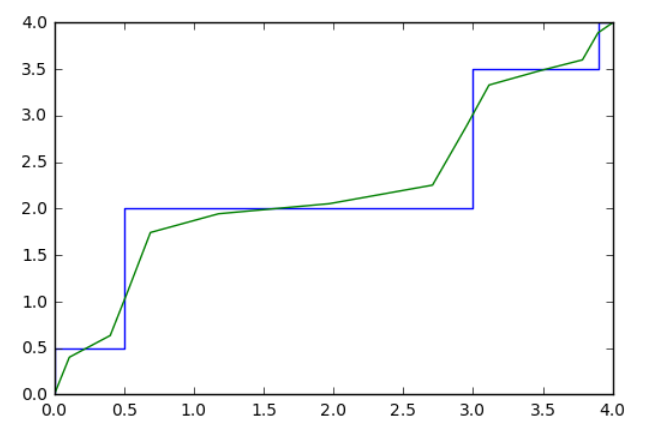
\includegraphics[width=\textwidth,height=6cm,keepaspectratio=true]{ejemplo_suavizado}
    \caption[Ejemplo de suavizado usando descenso gradiente]{Ejemplo de suavizado usando descenso gradiente. La línea azul representa un camino encontrado por el \Astar y la línea verde el resultado de aplicarle el suavizado}
    \label{fig:basics AFM sketch}
\end{figure}

\subsection{Eliminar el zigzag}

El primer método que hemos usado y que suele dar buenos resultados, es eliminar el zigzag. Este método es básicamente lo mismo que realiza el Theta* que explicaremos más adelante en \ref{referenciaTheta}.

El zigzag es el problema más habitual que nos hemos encontrado. Al representar un espacio continuo a través de casillas, se produce habitualmente porque aunque se use la representación octal permitiendo el movimiento diagonal, esto al pasarlo a un espacio no discreto quiere decir que sólo tenemos ocho posibles ángulos de movimiento: 0º, 45º, 90º, 135º, 180º, 225º, 270º y 315º

En realidad las posibilidades reales para movernos son cualquier ángulo de los 360º. Por tanto, si nuestro objetivo está en un ángulo diferente a esos ocho, se produce un zigzag combinándoles hasta que se consigue llegar.

La forma para eliminar el zigzag, es comprobar si es posible eliminar estos pasos intermedios. Es decir, si para llegar al objetivo, el \Astar ha usado varias casillas en el espacio discreto, es posible que en un espacio no discreto pudiéramos llegar directamente con un movimiento en un ángulo distinto a los ocho que permite el \Astar.

\begin{figure}[!htpb]
    \centering
    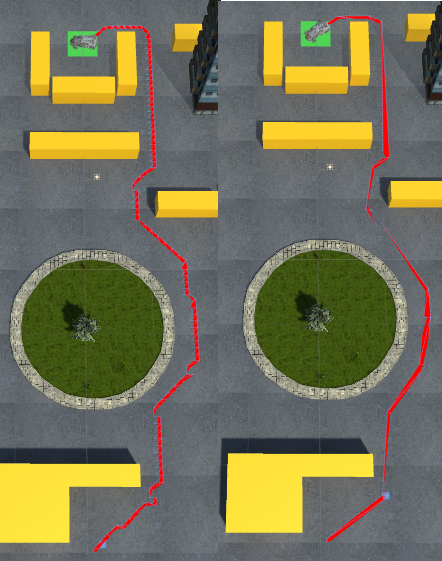
\includegraphics[width=\textwidth,height=11cm,keepaspectratio=true]{comparacion_a_star_zingzag}
    \caption[Comparación entre la ruta del \Astar con y sin zigzag]{A la izquierda la ruta obtenida con el \Astar, y a la derecha la ruta después de eliminar el zigzag.}
    \label{fig:basics AFM sketch}
\end{figure}

Para ello, usamos la línea de visión. Si existe una línea de visión entre una casilla del \Astar y otra quiere decir que podemos desplazarnos siguiendo una línea recta formada entre esas dos casillas. Con las casillas devueltas por el \Astar, comprobamos si existe línea de visión entre ellas. Entre casillas consecutivas siempre habrá línea de visión, porque si no, no sería un camino válido, pero puede también haber línea de visión entre las siguientes de forma que haya casillas sobrantes debido al zigzag y a la forma que tiene el \Astar de buscar el camino.

Así que lo que comprobamos es que existe una línea de visión entre una casilla del \Astar y la siguiente más lejana posible, y eliminamos a las casillas intermedias. De esta forma obtenemos una línea recta entre esas dos casillas y eliminamos el zigzag producido por las casillas intermedias.

\subsection{Descenso gradiente}

El descenso gradiente es un algoritmo iterativo de optimización que a partir de $N$ valores iniciales ($x_1, x_2, x_3, ..., x_n$), itera una función modificando esos valores gradualmente hacía un mínimo de una función $f(x_1, x_2, x_3, ..., x_n)$. El algoritmo termina cuando el cambio que se producen en los valores es menor que la tolerancia indicada.

Para optimizar la ruta, queremos obtener los valores que minimizan las distancia entre los puntos sucesivos de la ruta, y a su vez que minimicen las distancia a la ruta original.

Para minimizar la distancia entre los puntos con respecto a la ruta original usaremos las función:
\begin{center}
$y_i = y_i + \alpha (x_i - y_i)$
\end{center}
Donde $\alpha$ es el peso que le damos a cuanto de cerca queremos que la ruta suavizada esté de la ruta original, $x$ es el punto de la ruta original e $y$ es el nuevo punto suavizado.

Para minimizar la distancia entre los puntos sucesivos de la ruta, usamos la función:
\begin{center}
$y_i = y_i + \beta (y_{i+1} + y_{i-1} - 2 * y_i)$
\end{center}
Donde $\beta$ es el peso que le damos al suavizado de la ruta, y tenemos en cuenta la distancia tanto con el punto anterior como con el puto siguiente.

Para calcular el error que se produce, o el cambio hacia el mínimo, usamos la función:
\begin{center}
$error = error + (z_i - y_i)$
\end{center}
Donde $z$ es el valor de $y$ antes de calcular el nuevo mínimo.

En la figura 3.3 podemos ver los distintos resultados que obtenemos al usar distintos valores en $\alpha$ y $\beta$. El resultado que se observa más a la izquierda corresponde a $\alpha = 0.9$ y $\beta = 0.1$, con lo que obtenemos la ruta original. En el centro podemos ver el caso opuesto, con $\alpha = 0.0$ y $\beta = 0.3$, donde el camino más suavizado posible es la línea recta hasta la meta. Y por último, a la derecha, el resultado con $\alpha = 0.5$ y $\beta = 0.4$, que es bastante próximo al resultado de una ruta ideal.
\begin{figure}[!htpb]
    \centering
    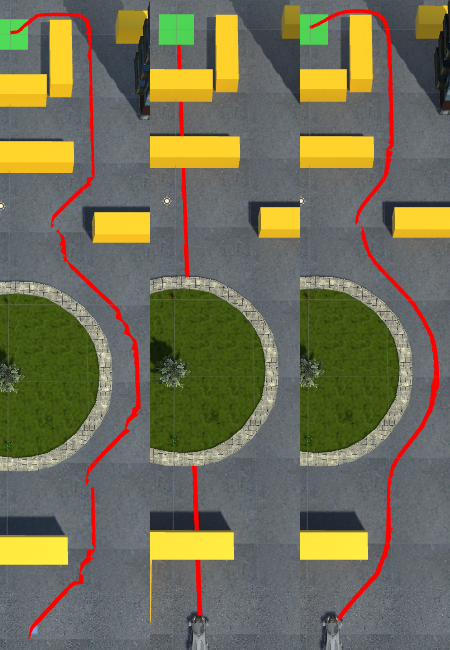
\includegraphics[width=\textwidth,height=11cm,keepaspectratio=true]{comparacion_a_star_descenso}
    \caption[Efecto de $\alpha$ y $\beta$ en el descenso gradiente]{Comparación entre los resultados del descenso gradiente con distintos $\alpha$ y $\beta$.}
    \label{fig:basics AFM sketch}
\end{figure}

\subsection{Curvas Bézier}
Las curvas Bézier \cite{bezierdevmag, wiki:bezier} son una forma de representar curvas a través de una función que recibe un parámetro. Hemos usado la función de las curvas de Bézier para suavizar la ruta y así obtener giros y curvas más cercanas a una representación real

Una función de una curva Bézier tiene varios puntos de control (al menos dos). De estos puntos, el primero y el último representan el inicio y el final de la curva. Esta función además recibe un parámetro que puede tomar los valores comprendidos entre cero y uno. Si el parámetro toma el valor cero, entonces la función devuelve el punto de inicio, mientras que si toma el valor uno devuelve el punto final. De esta forma, dando valores entre cero y uno, la función devuelve los valores que se encuentran entre los puntos de inicio y de fin.

Si la función toma dos puntos de referencia, lo que obtendremos sera una recta y sus puntos intermedios. Si la función toma tres puntos, entonces tendremos una curva donde el vértice será cercano al punto intermedio. Podemos usar más puntos para representar curvas más complejas o dar curvas con más variedad de formas.

\begin{figure}[htpb]
    \centering
    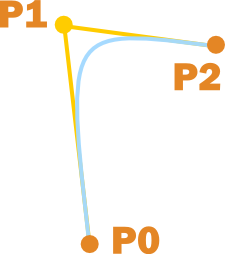
\includegraphics[width=\textwidth,height=6cm,keepaspectratio=true]{bezier_2_devmag}
    \caption[Esquema de una curva Bézier cuadrática de Herman Tulleken]{Esquema de una curva Bézier cuadrática de Herman Tulleken, Bézier Curves for your Games: A Tutorial \cite{bezierdevmag_imagen}.}
    \label{fig:basics AFM sketch}
\end{figure}

Hemos usado la función Bézier con tres puntos después de eliminar el zigzag, así que cada tres puntos del \Astar sin zigzag se usan como puntos de control que servirán para crear la curva. Si los puntos más o menos están alineados, el resultado será una recta suavizada, y si forman una curva, se eliminan los segmentos rectos y se reemplazan con puntos que forman una curva. 

La función Bézier cuadrática para tres puntos de control y parámetro $t$ es:

\begin{center}
$[x, y, z] = (1 – t)^2P_0 + 2(1 – t)tP_1 + t^2P_2$
\end{center}

En formato expandido:
\begin{center}
$x = (1 – t)^2x_0 + 2(1 – t)tx_1 + t^2x_2$

$y = (1 – t)^2y_0 + 2(1 – t)ty_1 + t^2y_2$

$z = (1 – t)^2z_0 + 2(1 – t)tz_1 + t^2z_2$
\end{center}

\begin{figure}[htpb]
    \centering
    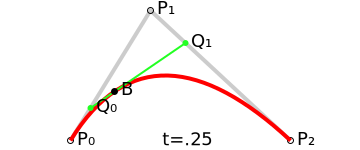
\includegraphics[width=\textwidth,height=6cm,keepaspectratio=true]{Bezier_2_wikipedia}
    \caption[Esquema de una curva Bézier cuadrática, Wikipedia]{Esquema de una curva Bézier cuadrática de Bézier curve --- Wikipedia \cite{wiki:bezierimagen}.}
    \label{fig:basics AFM sketch}
\end{figure}

\begin{figure}[!htpb]
    \centering
    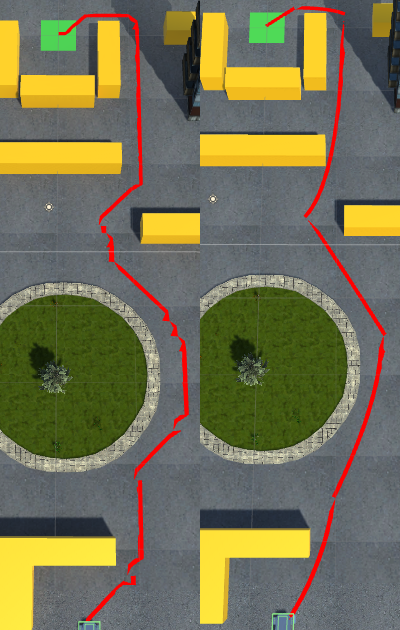
\includegraphics[width=\textwidth,height=9cm,keepaspectratio=true]{comparacion_a_star_bezier}
    \caption[Comparativa de rutas con \Astar y con curvas Bézier]{Comparación entre la ruta obtenida con el \Astar y con las curvas Bézier.}
    \label{fig:basics AFM sketch}
\end{figure}

\newpage

\section{Theta*} \label{referenciaTheta}
Theta* es un algoritmo desarrollado por A. Nash, K. Daniel, S. Koenig y A. Felner \cite{thetaestrella, thetaestrellaweb} en 2010 que modifica el \Astar original para obtener rutas más realistas.

Como explicamos anteriormente, el \Astar por la forma en la que representa el espacio de búsqueda, da resultados poco realistas, con lo que hay que realizar un postprocesado de la ruta obtenida. El Theta* incorpora este proceso al propio \Astar para obtener de forma directa rutas que no requieran del proceso de suavizado o que lo minimice.

Para ello, el cambio que hace el Theta* respecto al \Astar es que un sucesor a una casilla puede ser cualquier casilla, en vez de ser unicamente las que tiene alrededor. El algoritmo es el mismo que el \Astar original, pero cuando se calculan los sucesores, además de calcular si es un sucesor válido y el coste de ese sucesor, comprueba si hay línea de visión con la casilla del nodo padre del nodo que lo generó. Si no hay línea de visión, sigue el algoritmo del \Astar y le asigna al sucesor como padre la casilla que lo originó. Pero si hay línea de visión, le asigna como padre no el nodo que lo generó, sino el padre de este, calculando el coste del sucesor teniendo en cuenta esta otra casilla. De esta forma elimina las casillas intermedias que origina el \Astar que no son necesarias de forma similar a como se realizaría en el postprocesado para eliminar el zigzag.

Podemos observar el funcionamiento del algoritmo en la figura 3.7. La línea discontinua roja muestra el camino encontrado por el \Astar. En cambio, el Theta*, al haber una línea de visión entre el nodo $S_{start}$ y el nodo $S'$, le asigna como padre al nodo $S'$ el nodo $S_{start}$ sin pasar por el nodo intermedio $S$ como hace el \Astar.

\begin{figure}[htpb]
    \centering
    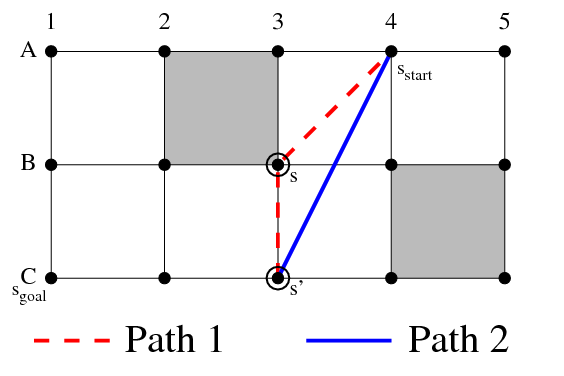
\includegraphics[width=\textwidth,height=5cm,keepaspectratio=true]{Theta_path_12}
    \caption[Comparación de los caminos elegidos por el \Astar y el Theta*]{Comparación de los caminos elegidos por el \Astar (path1) y el Theta* (path2) de \cite{thetaestrellawebimagen}.}
    \label{fig:basics AFM sketch}
\end{figure}

\section{\Astar con vértices} \label{avertices}
El algoritmo \Astar como hemos visto, divide el espacio de búsqueda en casillas de un espacio discreto. Esto presenta los problemas de rutas poco realistas, y además al ser discreto, no podemos representar una línea recta entre dos puntos distantes, si no que debemos recorrer todas las casillas intermedias.

Podemos mejorar ambos problemas usando un \textit{Nav Mesh} \ref{referenciaNavMesh}.  Un \textit{Nav Mesh}\footnote{\textit{Nav Mesh} es un conjunto de polígonos que se usan en los motores gráficos 3D para representar la zona recorrible de un agente} usa polígonos para representar el espacio de búsqueda de tal forma que los lados de estos polígonos y sus vértices se encuentran en los bordes del espacio recorrible, que es el espacio del mapa sin obstáculos por donde puede moverse en nuestro caso el vehículo. De esta forma, podemos usar esos vértices como las casillas del espacio discreto, lo que produce tres mejoras importantes:

\begin{enumerate}
\item La representación del espacio recorrible se ajusta más a un espacio continuo al poder ir de un vértice a otro sin pasar por estados intermedios.
\item Permite que las rutas obtenidas sean más realistas que las obtenidas con la representación discreta.
\item Al ser un espacio continuo dentro de los polígonos del \textit{Nav Mesh}, evitamos pasar por todos los estados intermedios de una representación discreta, reduciendo enormemente las casillas a explorar y reduciendo el tiempo de ejecución del algoritmo.
\end{enumerate}

Este algoritmo es una variante del \Astar, donde la función de sucesores cambia de los espacios contiguos a la casilla que se va a explorar, a los vértices que son visibles desde el la casilla actual. Las casillas ahora no son las contiguas si no que se encuentran en la posición de los vértices.

En la figura 3.8 podemos ver una comparación entre los sucesores generados por el \Astar, a la izquierda, y el \Astar usando los vértices, a la derecha. Las casillas rojas representan un obstáculo, la amarilla la casilla que se está explorando, y las casillas azules representan a los sucesores. Mientras que en el \Astar, los sucesores son las casillas contiguas, usando los vértices del \textit{Nav Mesh} evitamos las posiciones intermedias y obtenemos como sucesores las casillas visibles más alejadas desde la casilla que se está explorando.
\begin{figure}[htpb]
    \centering
    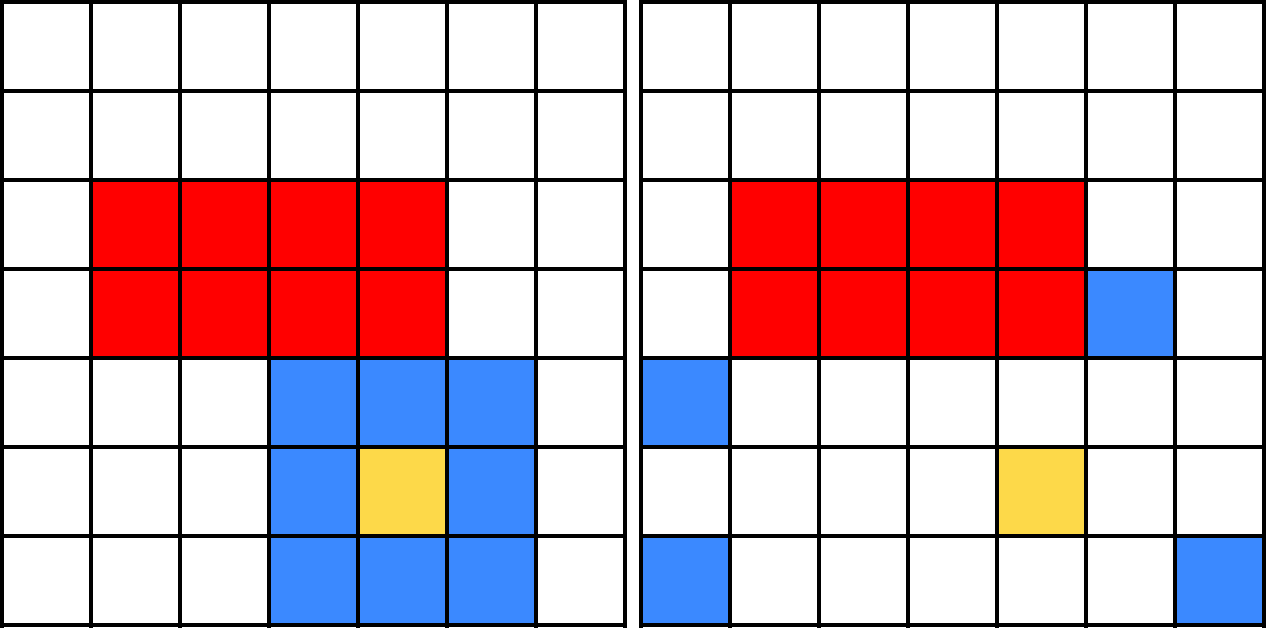
\includegraphics[width=\textwidth,height=5cm,keepaspectratio=true]{sucesoresVertices}
    \caption[Comparación entre los sucesores del \Astar y del \Astar usando los vértices]{Comparación entre los sucesores del \Astar y del \Astar usando los vértices. Las casilla rojas representan obstáculos, las amarillas la casilla que se está explorando y las casillas azules los sucesores.}
    \label{fig:basics AFM sketch}
\end{figure}

Podemos ver una comparativa con los resultados y tiempos del \Astar original en la sección Comparativa de los algoritmos \ref{comparativaAlgoritmos}.

\section{\textit{Hybrid \Astar}}
Los algoritmos que hemos visto anteriormente, tanto los que usan una representación totalmente discreta, hasta los que buscan aproximarse a rutas más realistas en un espacio continúo, tienen el problema de que no tienen en cuenta las características del vehículo que va a realizar la ruta.

El \textit{Hybrid \Astar}\cite{dolgov08gppISER,dolgov08gppSTAIR} se basa en el \Astar tradicional, pero teniendo en cuenta estos dos factores: que el vehículo se mueve por un espacio continuo, y que lo hace siguiendo sus limitaciones físicas.

Las limitaciones físicas definen dos tipos de vehículos, los holonómicos y los no holonómicos. Un vehículo es holonómico si es capaz de desplazarse en el mismo número de grados de libertad que el espacio donde se mueve. Por ejemplo, un coche se desplaza en un espacio con tres grados de libertad, dos para la posición y uno para la orientación. Pero en cambio sólo puede desplazarse a través de dos grados de libertad, uno de posición y otro de orientación, lo que le impide poder realizar movimientos laterales. Es por tanto un vehículo no holonómico. Para que fuese holonómico y no tener esa limitación, tendría que poder desplazarse en ese otro grado de libertad usando por ejemplo ruedas omnidireccionales.

El \textit{Hybrid \Astar}, utiliza una aproximación continua al \Astar. En nuestro caso, la aproximación usada ha sido el modelo de la bicicleta. Este modelo es válido porque los ejes de un vehículo son simétricos, por lo que el resultado de un lado del vehículo será equivalente al del otro lado, pudiéndolo simplificar como si fuera un solo eje formado por la rueda delantera y la rueda trasera.
\begin{figure}[htpb]
    \centering
    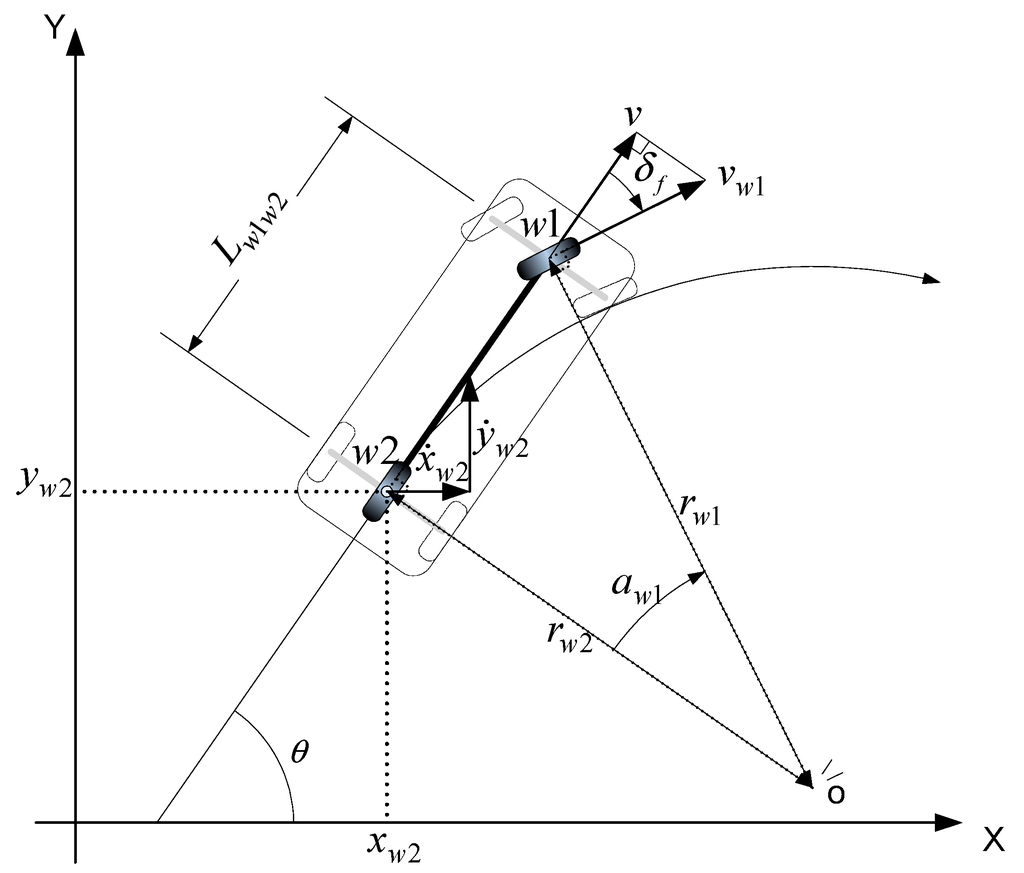
\includegraphics[width=\textwidth,height=10cm,keepaspectratio=true]{imagenmodelobicicleta}
    \caption[Esquema del modelo de la bicicleta]{Esquema del modelo de la bicicleta de \cite{articuloimagenmodelobicicleta}.}
    \label{fig:basics AFM sketch}
\end{figure}

Los elementos del modelo de la bicicleta son:
\begin{enumerate}
\item La rotación del vehículo $\theta$.
\item El ángulo de giro de las ruedas $\delta$
\item La distancia entre los ejes $L$
\item La distancia recorrida por el vehículo $d$
\end{enumerate}

Con estos elementos podemos calcular en que posición se encontrará el vehículo en un espacio de tiempo, teniendo en cuenta su capacidad de maniobra.

\label{formulashybrid}Las fórmulas para el cálculo de la nueva posición del vehículo son:
\begin{center}
$x' = x +  v \Delta t \sin \theta$

$z' = z +  v \Delta t \cos \theta$

$\theta' = \theta + \Delta t \omega $
\end{center}

Para $v \Delta t$ hemos realizado una aproximación, tal que hemos considerado que la velocidad del vehículo $v$ va a ser constante, y que $\Delta t$ es el tiempo que tarda en recorrer una unidad de nuestra representación. Esto es válido en nuestro caso y nos permite simplificar las ecuaciones porque la velocidad de nuestro vehículo a través del \textit{PID Controller} (ver sección \ref{pidcontroller}) va a ser aproximadamente constante. En un entorno real $v$ sería la velocidad del vehículo entre el lapso de tiempo recorrido entre las mediciones representado por $\Delta t$ 

Para calcular $\omega$, que es el radio de giro que realiza el vehículo en ese espacio de tiempo continuo, usamos la siguiente fórmula
\footnote{Norvig y Thrun «Intro to Artificial Intelligence» (\url{https://www.udacity.com/course/intro-to-artificial-intelligence--cs271}).}:
\begin{center}
$\omega = \displaystyle \frac{d}{L} * \tan \delta  $
\end{center}

Con estos elementos ya podemos calcular cual es el siguiente estado del vehículo en un espacio continuo. Los sucesores del estado actual serán esos estados continuos, variando el ángulo de giro, y podemos tener en cuenta el sentido permitiendo al vehículo ir marcha atrás añadiendo los sucesores correspondientes.

Esto nos permite además de obtener rutas más realistas, rutas que se adecuan a la maniobrabilidad del vehículo,  rutas que permiten maniobrar y cambiar de sentido si fuera necesario.

Una de las desventajas del \textit{Hybrid \Astar} es que no es un algoritmo completo, es decir que aunque exista una solución no siempre dará con ella, al contrario que el \Astar. Cuando calculamos los sucesores de un estado se asigna el mejor a una casilla discreta correspondiente del espacio discreto. Además, de forma tradicional el \textit{Hybrid \Astar} si vuelve a una casilla ya explorada, descarta ese camino. De esta forma, aunque en la mayoría de los casos encontrará un camino, no siempre lo hará aunque exista.

\subsection{Definición de los estados}
En el \Astar cada estado tenía asociado solamente la posición y su coste. En cambio en el \textit{Hybrid \Astar} necesitamos más parámetros para poder definir cada estado.

Los parámetros necesarios para cada estado el \textit{Hybrid \Astar} son:
\begin{itemize}
\item \textbf{Posición continua:} es la posición a donde se puede mover el vehículo teniendo en cuenta sus características y limitaciones.
\item \textbf{Posición discreta:} es la casilla del mapa representado de forma discreta que le corresponde a la posición continua.
\item \textbf{Orientación:} es el ángulo que forma el vehículo con el eje de referencia después de haber alcanzado la posición continua correspondiente.
\item \textbf{Sentido:} indica si el vehículo se tienen que mover hacia adelante o hacia atrás para alcanzar la posición.
\item \textbf{Coste:} es la suma del coste del camino hasta la posición continua más la estimación del camino hasta la meta.
\end{itemize}

\subsection{Función de sucesores}
Cuando con el \Astar calculamos los sucesores, cada uno de ellos corresponde a una posición discreta que a su vez corresponde a una casilla. Pero cuando calculamos lo sucesores de forma continua para el \textit{Hybrid \Astar} esto no ocurre.

A través de las fórmulas \ref{formulashybrid} para calcular la posición continua, podemos calcular tantos sucesores como se crea conveniente (mediante un parámetro del método). Tendremos un sucesor en línea recta hacía delante, y un sucesor en línea recta hacia atrás. Pero para los giros tendremos tantos como deseemos desde $0º$ hasta el ángulo máximo de giro de las ruedas del vehículo. Aunque cuantos más sucesores se decida calcular el coste computacional de la exploración será mucho mayor. Por ello, para este proyecto, se calculan seis sucesores correspondientes a los dos mencionados anteriormente, que van en línea recta adelante y atrás, y a los lados con el ángulo máximo de giro de las ruedas.

A continuación hay que asignar esos sucesores a una casilla discreta. Para ello tomamos el valor entero de su vector de posición, pero al hacer esto es posible que varios sucesores coincidan en la misma casilla discreta. En ese caso se elige aquel sucesor cuyo coste sea menor, descartando los otros. Es posible guardar todos los sucesores, el problema es el mismo que cuando se decide cuantos sucesores generar, el coste computacional sería muy alto debido a que el número de sucesores que se generaría con las posiciones continuas sería mucho mayor que su equivalente en una representación discreta. Descartando los peores sucesores continuos de cada posición discreta, contenemos el coste computacional.

\subsection{Cálculo del coste de la ruta} \label{hybridcoste}
El cálculo del coste a través de las funciones G() y H(), es la forma que tenemos de controlar como se va a realizar la búsqueda de la ruta, así como también que rutas se van a seleccionar con respecto a otras posibles.

Para el \textit{Hybrid \Astar} hemos ampliado la función G() para que además de la distancia euclídea entre un estado actual y su estado sucesor tenga en cuenta que::
\begin{enumerate}
\item Si el vehículo gira es un coste adicional.
\item Si el vehículo retrocede es un gran coste adicional
\item Si pasa cerca de un obstáculo es un coste adicional
\end{enumerate}

De esta manera se pretende que se seleccionen las rutas más realistas posibles. Por ejemplo, si no se penalizará el ir hacia atrás, podrían resultar casos donde el \textit{Hybrid \Astar} seleccionase una ruta donde fuese desde el inicio hasta la meta de forma continua marcha atrás, aunque pudiese girar e ir hacia adelante. Si ir marcha atrás es igual de válido que ir hacia adelante no habría motivo para dar la vuelta, pero ese resultado es poco realista debido a que en la realidad es peligroso y poco deseable ir marcha atrás más tiempo del necesario.

Al penalizar los giros ocurre un caso parecido puesto que en la realidad se prefiere ir en línea recta. Aunque, en este caso surge un conflicto con el tercer caso de mantener una distancia con los obstáculos. Es decir, a través de los pesos de la heurística el algoritmo debe decidir si es mejor girar y alejarse de un obstáculo o si es preferible mantenerse cerca pero ir en línea recta.

La fórmula utilizada para la función G() ha sido:
\begin{center}
$distanciaRecorrida = distanciaDesdeElPadre + distanciaPadre$

$pObstaculos = (100-(distanciaObstaculo/10))/100$

$coste = (distanciaRecorrida * pgiro * patras) * distanciaObstaculo$
\end{center}

Siendo $pgiro$ la penalización que se le aplica por realizar un giro, $patras$ la penalización que le aplica por ir marcha atrás y $pObstaculo$ la penalización por pasar cerca de un obstáculo.

\subsection{Mapa de distancias} \label{mapadistancias}
Cuando los algoritmos que hemos visto buscan la mejor ruta, a veces tienen el problema que el resultado que obtienen es un ruta que pasa demasiado próxima a los obstáculos. Puede ser debido a varios factores, como que la ruta más corta sea esa o que al realizar las heurísticas se haya preferido penalizar los giros para maximizar los tramos en que el vehículo sigue una línea recta evitando girar para alejarse de los obstáculos.

Pero normalmente no es conveniente que la ruta pase demasiado cerca de los obstáculos si no es necesario, para evitar que se produzcan choques, por ejemplo, al cambiar de dirección.

Para intentar evitar que se acerque demasiado, hemos utilizado dos métodos. Primero hemos dado un radio al \textit{Nav Mesh} de forma que no haya posiciones válidas demasiado cerca de los obstáculos. Y segundo, hemos creado un mapa de distancias que almacena la distancia de cada posición discreta al obstáculo más cercano. Al incorporar esta distancia a la función G(), el algoritmo prefiere posiciones que estén alejadas de los obstáculos.

\begin{figure}[htpb]
    \centering
    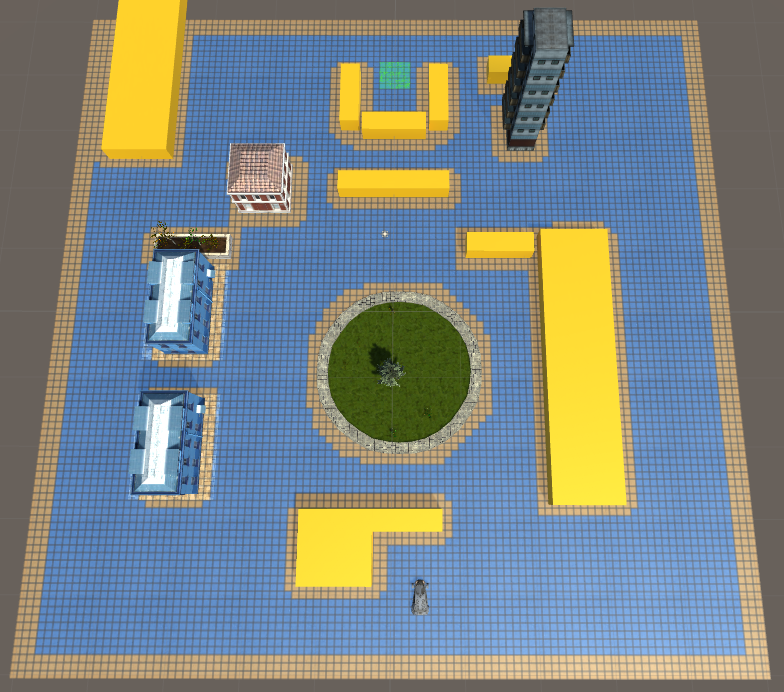
\includegraphics[width=\textwidth,height=10cm,keepaspectratio=true]{mapa_obstaculos}
    \caption[Representación del mapa de obstáculos]{Mapa de obstáculos: las casillas azules representan espacios libres, y las amarillas a los obstáculos una vez que se añadido una pequeña distancia de seguridad.}
    \label{fig:basics AFM sketch}
\end{figure}

Para crear el mapa de distancias, primero hemos creado un mapa de los obstáculos. Para ello hemos usado el \textit{Nav Mesh} para generar una matriz con las casillas libre y las ocupadas. Iterando a través de todas las posiciones discretas hemos comprobado con el \textit{Nav Mesh} si correspondían a una casilla recorrible o no.

A partir del mapa de obstáculos hemos creado el mapa de distancias\label{mapaobstaculos}. Hemos utilizado el algoritmo \textit{BrushFire} o \textit{GrassFire}. Este algoritmo parte desde una posición inicial a la que asigna un valor, generalmente cero, y asigna o actualiza a todas las posiciones adyacentes a su valor más uno. A continuación realiza el mismo proceso con esas posiciones adyacentes. De está manera, partiendo desde las casillas de los obstáculos, podemos actualizar la distancia a la que se encuentran de ese obstáculo y crear el mapa de las distancias.

Primero se inicializa con un valor máximo a todas las casillas. Una vez inicializado el mapa de distancias, partiendo de los obstáculos a los que se les asigna el valor cero, se recorre las casillas adyacentes que se actualizará su distancia al valor de la casilla previa más uno. Si una casilla ya ha sido actualizada previamente, se le asignará el valor menor que corresponde a la distancia al obstáculo más cercano.

\begin{figure}[htpb]
    \centering
    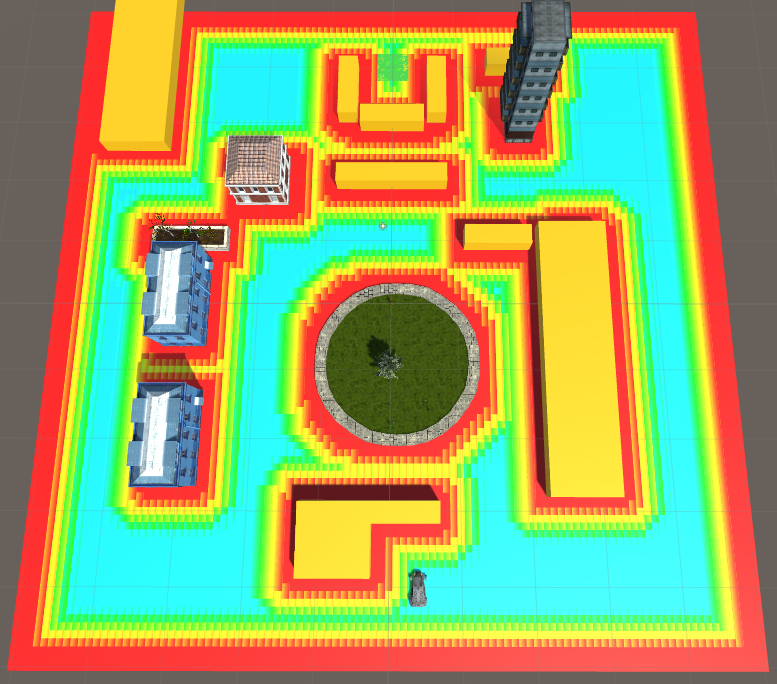
\includegraphics[width=\textwidth,height=10cm,keepaspectratio=true]{mapa_distancias}
    \caption[Representación del mapa de distancias]{Mapa de distancias: los colores hacia el rojo representan cercanía a un obstáculo, y los colores cercanos al azul y verde casillas alejadas.}
    \label{fig:basics AFM sketch}
\end{figure}

%\clearpage
\subsubsection{Pseudocódigo \textit{BrushFire} o \textit{GrassFire}} \label{brushfire}
\scalebox{1.0}{
\begin{algorithm}[H]
	abiertos = $\O$\;

    \ForAll{las casillas del mapa de distancias}{
    		casilla.distancia = valorMáximo\;
    }
    
    \ForAll{los obstáculos en el mapa de obstáculos} {
    		obstáculos.distancia = 0\;
    		mapaDistancias.actualizar(obstáculo, obstáculo.distancia)\;
    		abiertos.añadir(obstáculo)\;
    	}

	\While{abiertos no esté vacío}{
		actual = abiertos.primero()\;
		
		sucesores = obtenerSucesores(actual)\;
		
		\ForAll{los sucesores de actual} {
			\If {sucesor no es obstáculo}{
				sucesor.distancia = actual.distancia + 1\;
				anterior = mapaDistancias(sucesor)\;
				
				\If {anterior.distancia $>$ sucesor.distancia}{
					mapaDistancias.actualizar(sucesor, sucesor.distancia)\;
			    		abiertos.añadir(sucesor)\;
				}
			}
		}
	}

 \caption{Pseudocódigo del \textit{BrushFire} o \textit{GrassFire}}
\end{algorithm}
}

\subsection{Heurística \textit{Hybrid \Astar}} \label{hueristicahybrid}
Una estrategia común para obtener heurísticas es relajar las condiciones que determinan la distancia en el mundo real. Para la realización de la función heurística podemos considerar tres posibilidades principalmente:

\begin{enumerate}
\item La distancia euclídea en línea recta desde las posición actual hasta la meta.
\item La distancia hasta la meta teniendo en cuenta los obstáculos que se encuentren pero sin tener en cuenta las restricciones de movimiento.
\item La distancia hasta la meta sin tener en cuenta los obstáculos pero teniendo en cuenta las restricciones de movimiento.
\end{enumerate}

Todos estos casos son una simplificación del caso real, debido a que la función heurística es una estimación del coste y como vimos en la heurística del \Astar \ref{heuristicaaestrella}, para que el algoritmo sea admisible no se debe sobreestimar el coste hasta la meta.

Para este proyecto hemos usado la heurística del segundo caso, y hemos precalculado el coste desde todos los posibles estados hasta la meta teniendo en cuenta los obstáculos que se encuentran en el mapa. Para ello, hemos usado el mapa de obstáculos \ref{mapaobstaculos} que generamos previamente, y usando el algoritmo \textit{Brushfire o Grassfire} \ref{brushfire} desde la meta, hemos guardado un mapa con las distancias de cada estado hasta la meta dando a las casillas de obstáculos un valor máximo.

De esta forma conseguimos mejorar el coste computacional del \textit{Hybrid \Astar} puesto que la estimación del coste del camino hasta la meta, se acerca más al coste real aún no teniendo en cuenta las limitaciones del movimiento, consiguiendo reducir el número de estados a explorar.

\section{\textit{PID Controller}}\label{pidcontroller}
Para mover el vehículo vamos a usar un \textit{PID Controller} (Controlador Proporcional, Integral y Diferencial). Un controlador de este tipo itera y se retroalimenta para corregir el error existente entre el valor actual y el resultado que se quiere conseguir.

Este algoritmo se usa para conseguir que el vehículo siga la ruta planificada lo más fielmente posible y es posible usarlo con cualquiera de los algoritmos anteriores. En nuestro caso, comprueba en cada momento el error que existe entre la posición del vehículo y la ruta obtenida con los algoritmos para obtener el giro del volante necesario.

La parte \textbf{proporcional} considera la diferencia entre el valor actual y el valor objetivo, y aplica la corrección (la fuerza que debe hacer un motor, o el ángulo de giro de las ruedas) de forma proporcional a ese error. El problema con la parte \textbf{proporcional} es que puede excederse. Es decir, al acercarse al valor correcto utilizar una corrección excesiva que haga que sobrepase el valor correcto, y tenga que corregirse en sentido contrario a continuación. El efecto de solo considerar la parte \textbf{proporcional} sería un vehículo balanceándose de un lado al otro de la ruta que intenta seguir.

La parte \textbf{diferencial} sirve para corregir el exceso que se puede producir en la parte \textbf{proporcional}. No tiene en cuenta el error si no su variación en el tiempo e intenta que esta variación sea continua en el tiempo. De esta forma, cuando se acerca al valor deseado suaviza la corrección que produce la parte \textbf{proporcional}, y si nos excedemos evita que se realice una corrección brusca en el otro sentido. Así evita que el controlador balancee alrededor del valor objetivo y se acerque de una forma estable.

La parte \textbf{integral} se encarga de corregir el error que se produce por causas externas. Por ejemplo, si en un vehículo se produce siempre un sobregiro hacia un lado por una avería o alguna otra causa, la parte \textbf{integral} se encarga de añadir la corrección necesaria para compensarlo. Para ello no considera sólo el error, si no como se ha mantenido a lo largo del tiempo. Si un error persiste e impide acercarnos al objetivo, la parte \textbf{integral} intentará compensarlo. Por ejemplo, en el caso del vehículo con un problema de sobregiro, aplicará una corrección a la parte \textbf{proporcional} para compensar el sobregiro y que no gire en exceso las ruedas.

\begin{figure}[htpb]
    \centering
    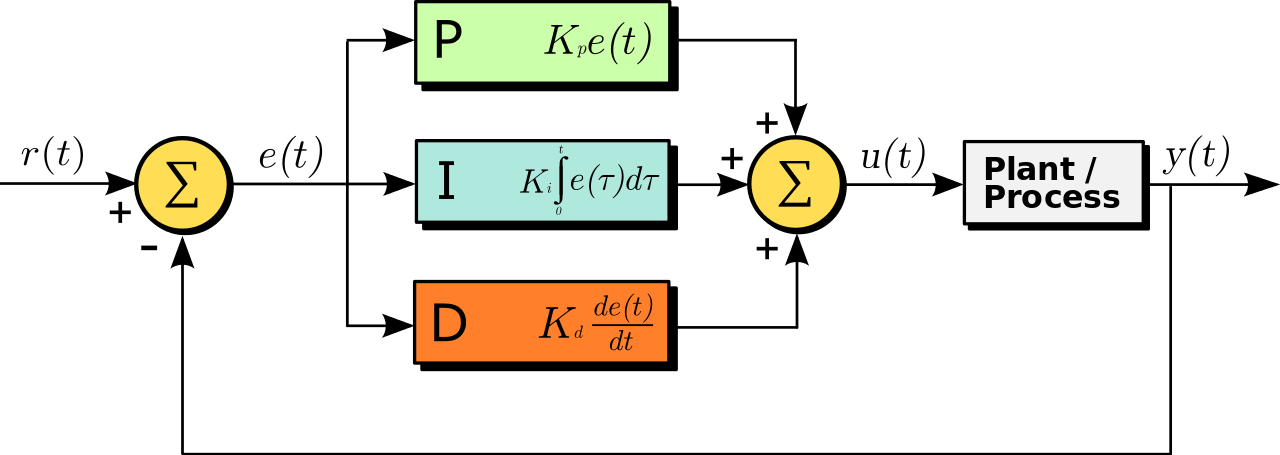
\includegraphics[width=\textwidth,height=10cm,keepaspectratio=true]{PID_wikipedia}
    \caption[Esquema de un \textit{PID controller}]{Esquema de un \textit{PID controller} de \cite{wiki:pidimagen}.}
    \label{fig:basics AFM sketch}
\end{figure}

Cada parte del controlador recibe un parámetro que controla cuanto afecta al resultado. Normalmente queremos que la mayor parte del resultado venga establecido por el a parte \textbf{proporcional}, dando valores bajos tanto a la parte \textbf{diferencial} como a la \textbf{integral}. Si se diese un peso alto a la parte \textbf{diferencial} podría producir el efecto contrario al que pretende evitar y excederse. Si se diese un peso alto a la parte \textbf{integral}, podría producir un estado inestable debido al error acumulado a lo largo del tiempo.

Las fórmulas de un PID Controller son las siguiente:
\begin{center}
$P = paramP * (valorObjetivo(t) - valorActual(t))$

$I = paramI * \left(\displaystyle \int_{0}^{t} errorAcumulado(t) dt\right)$

$D = paramD * \left(\displaystyle \frac{errorAnterior(t)-errorActual(t)}{dt}\right)$
\end{center}

Y el valor final que se usará para corregir el valor actual y acercarnos al valor objetivo lo obtenemos sumando los tres resultados:
\begin{center}
$error = P + I + D$
\end{center}